%%%%%%%%%%%%%%%%%%%%%%%%%%%%%%%%%%%%%%%%%%%%%%%%%%%%%%%%%%%%%%%%%
% \documentclass[hyperref={pdfpagelabels=false},compress,table]{beamer} % 在Mac下无法编译
\documentclass[compress,table]{beamer} % 在Mac下使用
% package for font
\usepackage{fontspec}
\defaultfontfeatures{Mapping=tex-text}  %%如果没有它,会有一些 tex 特殊字符无法正常使用,比如连字符。
\usepackage{xunicode,xltxtra}
\usepackage[BoldFont,SlantFont,CJKnumber,CJKchecksingle]{xeCJK}  % \CJKnumber{12345}: 一万二千三百四十五
\usepackage{CJKfntef}  %%实现对汉字加点、下划线等。
\usepackage{pifont}  % \ding{}
% package for math
\usepackage{amsfonts}

% package for graphics
\usepackage[americaninductors,europeanresistors]{circuitikz}
\usepackage{tikz}
\usetikzlibrary{plotmarks}  % placements=positioning
\usepackage{graphicx}  % \includegraphics[]{}
\usepackage{subfigure}  %%图形或表格并排排列
% package for table
\usepackage{colortbl,dcolumn}  %% 彩色表格
\usepackage{multirow}
\usepackage{multicol}
\usepackage{booktabs}
% package for code
\usepackage{fancyvrb}
\usepackage{listings}

% \usepackage{animate}
% \usepackage{movie15}

%%%%%
% setting for beamer
\usetheme{default} % Madrid(常用), Copenhagen, AnnArbor, boxes(白色), Frankfurt,Berkeley
\useoutertheme[subsection=true]{miniframes} % 使用Berkeley时注释本行
\usecolortheme{sidebartab}
\usefonttheme{serif}  %%英文使用衬线字体
% \setbeamertemplate{background canvas}[vertical
% shading][bottom=white,top=structure.fg!7] %%背景色,上25%的蓝,过渡到下白。
\setbeamertemplate{theorems}[numbered]
\setbeamertemplate{navigation symbols}{}  %% 去掉页面下方默认的导航条
\setbeamercovered{transparent}  %设置 beamer 覆盖效果

% 设置标题title背景色
% \setbeamercolor{title}{fg=black, bg=lightgray!60!white}
\setbeamercolor{title}{fg=white, bg=black!70!white}

% 设置每页小LOGO
\pgfdeclareimage[width=1cm]{ouc}{figures/static/ouc.pdf}
\logo{\pgfuseimage{ouc}{\vspace{-20pt}}}

% setting for font
%%\setCJKmainfont{Adobe Kaiti Std}
\setCJKmainfont{SimSun} 
%% \setCJKmainfont{FangSong_GB2312} 
%% \setmainfont{Apple Garamond}  %%苹果字体没有SmallCaps
\setCJKmainfont{SimSun} 
%FUNNY%\setCJKmainfont{DFPShaoNvW5-GB}  %%华康少女文字W5(P)
%FUNNY%\setCJKmainfont{FZJingLeiS-R-GB}  %%方正静蕾体
%FUNNY%\setmainfont{Purisa}
%\setsansfont[Mapping=tex-text]{Adobe Song Std}
     %如果装了Adobe Acrobat,可在font.conf中配置Adobe字体的路径以使用其中文字体。
     %也可直接使用系统中的中文字体如SimSun、SimHei、微软雅黑等。
     %原来beamer用的字体是sans family;注意Mapping的大小写,不能写错。
     %设置字体时也可以直接用字体名,以下三种方式等同:
     %\setromanfont[BoldFont={黑体}]{宋体}
     %\setromanfont[BoldFont={SimHei}]{SimSun}
     %\setromanfont[BoldFont={"[simhei.ttf]"}]{"[simsun.ttc]"}
% setting for graphics
\graphicspath{{figures/}}  %%图片路径
\renewcommand\figurename{图}

% setting for pdf
\hypersetup{% pdfpagemode=FullScreen,%
            pdfauthor={Xiaodong Wang},%
            pdftitle={Title},%
            CJKbookmarks=true,%
            bookmarksnumbered=true,%
            bookmarksopen=false,%
            plainpages=false,%
            colorlinks=true,%
            citecolor=green,%
            filecolor=magenta,%
            linkcolor=blue,%red(default)
            urlcolor=cyan}

% setting for fontspec
\XeTeXlinebreaklocale "zh"  %%表示用中文的断行
\XeTeXlinebreakskip = 0pt plus 1pt minus 0.1pt  %%多一点调整的空间
%%%%%

% font setting by xeCJK
\setCJKfamilyfont{NSimSun}{NSimSun}
\newcommand{\song}{\CJKfamily{NSimSun}}
%%%\setCJKfamilyfont{AdobeSongStd}{Adobe Song Std}
%%%\newcommand{\AdobeSong}{\CJKfamily{AdobeSongStd}}
\setCJKfamilyfont{FangSong}{FangSong_GB2312}
\newcommand{\fang}{\CJKfamily{FangSong}}
%%%\setCJKfamilyfont{AdobeFangsongStd}{Adobe Fangsong Std}
%%%\newcommand{\AdobeFang}{\CJKfamily{AdobeFangsongStd}}
\setCJKfamilyfont{SimHei}{SimHei}
\newcommand{\hei}{\CJKfamily{SimHei}}
%%%\setCJKfamilyfont{AdobeHeitiStd}{Adobe Heiti Std}
%%%\newcommand{\AdobeHei}{\CJKfamily{AdobeHeitiStd}}
\setCJKfamilyfont{KaiTi}{KaiTi}
\newcommand{\kai}{\CJKfamily{KaiTi}}
%%%\setCJKfamilyfont{AdobeKaitiStd}{Adobe Kaiti Std}
\newcommand{\AdobeKai}{\CJKfamily{AdobeKaitiStd}}
\setCJKfamilyfont{LiSu}{LiSu}
\newcommand{\li}{\CJKfamily{LiSu}}
\setCJKfamilyfont{YouYuan}{YouYuan}
\newcommand{\you}{\CJKfamily{YouYuan}}
\setCJKfamilyfont{FZJingLei}{FZJingLeiS-R-GB}
\newcommand{\jinglei}{\CJKfamily{FZJingLei}}
\setCJKfamilyfont{MSYH}{Microsoft YaHei}
\newcommand{\msyh}{\CJKfamily{MSYH}}

% 自定义颜色
\def\Red{\color{red}}
\def\Green{\color{green}}
\def\Blue{\color{blue}}
\def\Mage{\color{magenta}}
\def\Cyan{\color{cyan}}
\def\Brown{\color{brown}}
\def\White{\color{white}}
\def\Black{\color{black}}

\lstnewenvironment{javaCode}[1][]{% for Java
  \lstset{
    basicstyle=\tiny\ttfamily,%
    columns=flexible,%
    framexleftmargin=.7mm, %
    frame=shadowbox,%
    rulesepcolor=\color{cyan},%
    % frame=single,%
    backgroundcolor=\color{white},%
    xleftmargin=4\fboxsep,%
    xrightmargin=4\fboxsep,%
    numbers=left,numberstyle=\tiny,%
    numberblanklines=false,numbersep=7pt,%
    language=Java, %
    }\lstset{#1}}{}

\lstnewenvironment{shCode}[1][]{% for Java
  \lstset{
    basicstyle=\scriptsize\ttfamily,%
    columns=flexible,%
    framexleftmargin=.7mm, %
    frame=shadowbox,%
    rulesepcolor=\color{brown},%
    % frame=single,%
    backgroundcolor=\color{white},%
    xleftmargin=4\fboxsep,%
    xrightmargin=4\fboxsep,%
    numbers=left,numberstyle=\tiny,%
    numberblanklines=false,numbersep=7pt,%
    language=sh, %
    }\lstset{#1}}{}

\newcommand\ask[1]{\vskip 4bp \tikz \node[rectangle,rounded corners,minimum size=6mm,
  fill=white,]{\Cyan \includegraphics[height=1.5cm]{question} \Large \msyh #1};}

\newcommand\wxd[1]{\vskip 4bp \tikz \node[rectangle,minimum size=6mm,
  fill=blue!60!white,]{\White \ding{118} \msyh #1};}

\newcommand\xyy[1]{\vskip 2bp \tikz \node[rectangle,minimum size=3mm,
  fill=black!80!white,]{\White \msyh\scriptsize #1};}

\newcommand\cxf[1]{\vskip 4bp \tikz \node[rectangle,rounded corners,minimum size=6mm,
  fill=orange!60!white,]{\White \ding{42} \msyh #1};}

\newcommand\samp[1]{\vskip 2bp \tikz \node[rectangle,minimum size=3mm,
  fill=white!100!white,]{\Mage\msyh \small CODE \ding{231} \Black #1};\vskip -8bp}

\newcommand\zhyfly[1]{\tikz \node[rectangle,rounded corners,minimum size=6mm,ball
  color=red!25!blue,text=white,]{#1};}

\newcommand\pno[1]{\tikz \node[rectangle,rounded corners,minimum size=1mm,
  fill=yellow!50!black,text=white,]{\msyh\scriptsize P. #1};}

\setbeamerfont{frametitle}{series=\msyh} % 修改Beamer标题字体

\makeatletter
\newcommand{\Extend}[5]{\ext@arrow 0099{\arrowfill@#1#2#3}{#4}{#5}}
\makeatother
%%%%%%%%%%%%%%%%%%%%%%%%%%%%%%%%%%%%%%%%%%%%%%%%%%%%%%%%%%%%%%%%%

%%%%%%%%%%%%%%%%%%%%%%%%%%%%%%%%%%%%%%%%%%%%%%%%
% \titlepage
\title[KevinW@OUC]{\hei {\huge Java 应用程序设计}\\  
  泛型}
\author[王晓东]{王晓东\\
  \href{mailto:wxd2870@163.com}{\footnotesize wxd2870@163.com}}
\institute[中国海洋大学]{\small 中国海洋大学}
\date{\today}
\titlegraphic{\vspace{-6em}
\includegraphics[height=6cm]{static/ouc.pdf}\vspace{-6em}}
%%%%%
\begin{document}
%% Delete this, if you do not want the table of contents to pop up at
%% the beginning of each subsection:
\AtBeginSection[]{                              % 在每个Section前都会加入的Frame
  \frame<handout:0>{
    \frametitle{\textbf{\hei 接下来…}}
    \tableofcontents[currentsection]
  }
}  %

\AtBeginSubsection[]                            % 在每个子段落之前
{
  \frame<handout:0>                             % handout:0 表示只在手稿中出现
  {
    \frametitle{\textit{\hei 接下来…}}\small
    \tableofcontents[current,currentsubsection] % 显示在目录中加亮的当前章节
  }
}
 \frame{\titlepage}

%%%%%%%%%%%%%%%%%%%%%%%%%%%%%%%%%%%%%%%%%%%%%%%%
\begin{frame}
\frametitle{参考书目}
\begin{enumerate}
\item 张利国、刘伟[编著], Java SE应用程序设计, 北京理工大学出版社, 2007.10.

\end{enumerate}  
\end{frame}

\begin{frame}
\frametitle{本章学习目标}
\begin{enumerate}
\item 什么是泛型
\item 使用泛型
  \begin{itemize}
  \item 集合框架中的泛型
  \item 泛型的向后兼容性
  \end{itemize}
\item 泛型进阶
  \begin{itemize}
  \item 类型参数 / 定义自己的泛型类
  \item 类型通配符
  \item 泛型方法
  \item  受限制的类型参数
  \end{itemize}
\end{enumerate}  
\end{frame}

\section*{大纲}
\frame{\frametitle{大纲} \tableofcontents }

\section{泛型}
\begin{frame}[fragile] % [fragile]参数使得能够插入代码
\frametitle{什么是泛型}
泛型(Gernerics)机制自JDK 5.0开始引入,其实质是将原本确定不变的数据类型参数化。

\xyy{泛型优势}\\
作为对原有Java类型体系的扩充,使用泛型可以提高Java应用程序的类型安全、可维护性和可
靠性。

\end{frame}

\begin{frame}[fragile] % [fragile]参数使得能够插入代码
\frametitle{泛型分析}

\wxd{集合框架中的数据造型问题}\\

传统的集合为了提供广泛的适用性,会将所有加入其中的元素当作Object类型来处理,如Vector集合。
基于此原因,在实际使用时,我们必须将从集合中取出的元素值再强制转换为所期望的类型。
\xyy{无泛型机制}
\begin{javaCode}
Vector v = new Vector();
v.addElement(new Person("Tom", 18));
Person p = (Person)v.elementAt(0);
p.showInfo();
\end{javaCode}

{\Mage\it 泛型允许编译器实施由开发者设定的附加类型约束,将类型检查从运行时挪到编译时进行,这样类型
错误就可以在编译时暴露出来、而不是在运行时才发作(抛出ClassCastException运行异常)。}
\end{frame}

\section{使用泛型}
\begin{frame}[fragile] % [fragile]参数使得能够插入代码
\frametitle{集合框架中的泛型}
\wxd{用法}

创建集合容器时规定其允许保存的元素类型,然后由编译器负责添加元素的类型合法性检查,在取用
集合元素时则不必再进行造型处理。

\xyy{使用泛型的列表集合}
\begin{javaCode}
import java.util.Vector;
import java.util.Data;

public class TestVector {
  public static void main(String[] args) {
    Vector<String> v = new Vector<String>();
    v.addElement("Tom");
    v.addElement("Nancy");
    v.addElement("new Data()");  //编译时出错
    v.addElement("new Integer(300)");  //编译时出错

    for(int i = 0; i < v.size(); i++) {
      String name = v.elementAt(i); //并不需要进行强制类型转换
      System.out.println(name);
    }
  }
}
\end{javaCode}
\end{frame}

\begin{frame}[fragile] % [fragile]参数使得能够插入代码
\frametitle{集合框架中的泛型}

\xyy{在Hashtable中使用泛型}\\
\samp{Employee.java}
\begin{javaCode}
public class Employee {
  private final int id;
  private String name;
  private double salary;

  public Employee(int id, String name, double salary) {
    this.id = id;
    this.name = name;
    this.salary = salary;
  }
  // ...
  public void showInfo() {
    System.out.println(id + "\t" + name + "\t" + salary);
  }
}
\end{javaCode}
\end{frame}

\begin{frame}[fragile] % [fragile]参数使得能够插入代码
\frametitle{集合框架中的泛型}

\samp{TestHashtable.java}
\begin{javaCode}
import java.util.Hashtable;

public class Testhashtable {
  public static void main(String[] args) {
    Hashtable<Integer, Employee> ht = new Hashtable<Integer, Employee>();
    ht.put(101, new Employee(101, "张三", 5000));
    ht.put(102, new Employee(102, "李四", 4800));

    Employee e = ht.get(102);
    e.showInfo();
  }
}
\end{javaCode}

程序中直接将int型数据当作映射“键”使用,是由于Java的自动封装机制——系统已自动将int型数据值
转换为Integer类型对象。
\end{frame}

\begin{frame}[fragile] % [fragile]参数使得能够插入代码
\frametitle{泛型的向后兼容性}

Java语言中的泛型是维护向后兼容的,我们完全可以不采用泛型、而继续沿用过去的做法。这些未加
改造的旧式代码将无法享用泛型带来的便利和安全性。
\end{frame}


\begin{frame}[fragile] % [fragile]参数使得能够插入代码
\frametitle{泛型的向后兼容性}

Java语言中的泛型向过去兼容在高版本开发环境中编译未启用泛型机制的集合框加应用代码时,会输
出类似于如下形式的编译提示信息:
\begin{stdoutCode}
注意: /home/xiaodong/JavaTest/TestArrayList.java
使用了未经检查或不安全的操作。
注意: 要了解详细信息,请使用 -Xlint:unchecked 重新编译。
\end{stdoutCode}

可以使用SuppressWarnings注解关闭编译提示或警告信息:
\begin{javaCode}
@SuppressWarnings({"unchecked"})  
public class TestSuppressWarnings {
  //
}
\end{javaCode}
\end{frame}

\section{泛型进阶}

\begin{frame}[fragile] % [fragile]参数使得能够插入代码
\frametitle{类型参数}

如Vector<String>,其中,尖括号括起来的部分被称为{\hei 类型参数},而这种由类型参数修饰的类
型则被称为{\hei 泛型类},我们可以将泛型类理解为一种新的构造类型,当然也一定属于引用类型。

\emph{注意:应在声明泛型类变量和创建对象时均给出类型参数,且两者应保持一致。}

\end{frame}

\begin{frame}[fragile] % [fragile]参数使得能够插入代码
\frametitle{类型参数}

使用类型参数E进行泛型化处理的java.util.Vector类的定义代码摘要如下:
\begin{javaCode}
public class Vector<E> --- {
  public void addElement(E obj) { --- }
  public E elementAt(int index) { --- }
}  
\end{javaCode}
这里的E也称为“形式类型”参数。在实际使用该泛型类时,我们需要指定相应的具体类型,即实际类型参数。
\begin{javaCode}
Vector<String> v = new Vector<String>();  
\end{javaCode}

编译器遇到Vector<String>类型变量时,即知道此Vector变量/对象的类型参数E已经被绑定为String类型,进而也就确定其addElement()方法的参数和elementAt()方法的返回值均为String类型。

\end{frame}

\begin{frame}[fragile] % [fragile]参数使得能够插入代码
\frametitle{类型参数}
\xyy{使用自己的泛型类}\\
\samp{Person.java}
\begin{javaCode}
public class Person<T> {
  private final int id;
  private T secrecy;
  public Person(int id) {
    this.id = id;
  }
  public getId() {
    return id;
  }
  public void setSecrecy(T secrecy) {
    this.secrecy = secrecy;
  }
  public T getSecrecy() {
    return secrecy;
  }
}  
\end{javaCode}
\end{frame}

\begin{frame}[fragile] % [fragile]参数使得能够插入代码
\frametitle{类型参数}
\samp{Test.java}
\begin{javaCode}
public class Test {
  public static void main(String[] args) {
    Person<String> p1 = new Person<String>(101);
    p1.setSecrecy("芝麻开门");
    String s = p1.getSecrecy();
    System.out.println(p1.getId() + "\t 密码是:" + s);
  
    Person<Double> p2 = new Person<Double>(102);
    p2.setSecrecy("8700.85");
    double money = p2.getSecrecy();
    System.out.println(p2.getId() + "\t 秘密资金数额是:" + money);
}
\end{javaCode}

上述代码示例中的泛型类Person可以在使用时通过类型参数T指定其属性secrecy的具体类型(以及该
属性相应存/取方法的参数和返回值类型),进而提供了通用的信息存储能力。
\end{frame}

\begin{frame}[fragile] % [fragile]参数使得能够插入代码
\frametitle{类型参数}

形式类型参数的编程惯例。
\wxd{Java编程惯例}\\
\begin{table}
\footnotesize
\setlength{\extrarowheight}{1.2mm}
\rowcolors[]{1}{blue!20}{blue!10}
\begin{tabular}{c|p{6cm}}
{\bf 符号} & {\bf 意义}  \\
K & 键,比如映射的键\\
V & 值,比如List和Set的内容,或者Map中的值\\
E & 元素,比如Vector<E>\\
T & 泛型\\
\end{tabular}
\end{table}
\end{frame}

\begin{frame}[fragile] % [fragile]参数使得能够插入代码
\frametitle{类型通配符}
\wxd{对泛型的理解}
\begin{itemize}
\item 泛型类可以理解为具有广泛适用性、尚未最终定型的类型。
\item Person<String>和Person<Double>属于同一个类,但确是不同的类型。
\item 同一个泛型类与不同的类型参数复合而成的类型间并不存在继承关系,即使是类型参数间存在
  继承关系时也是如此。\\
  如:Vector<String>不是Vector<Object>的子类。
\end{itemize}
\end{frame}

\begin{frame}[fragile] % [fragile]参数使得能够插入代码
\frametitle{泛型类型的处理}

\xyy{遍历泛型Vector集合}

\begin{javaCode}
public void overview(Vector<String> v) {
  for(String o: v) {
    String.out.println(o);
  }
}
\end{javaCode}

上述方法用于遍历Vector<String>类型集合。但,我们可能还需要定义多个类似的方法来遍历其他类型的Vector集合元素。例如,定义overview(Vector<Person> v)、overview(Vector<Integer> v)等,显然过于繁琐,引用泛型机制后代码的通用性似乎不如从前。
\end{frame}

\begin{frame}[fragile] % [fragile]参数使得能够插入代码
\frametitle{泛型类型的处理}

一种可能的处理方法:将遍历方法的形参定义为不带任何类型参数的原型类型Vector,但这样会破坏已有的类型安全性。

\begin{javaCode}
public void overview(Vector v) {
  for(Object o: v) {
    String.out.println(o);
  }
}
\end{javaCode}

上述代码能够编译和运行,但编译时会出现“unchecked”提示信息。
\end{frame}

\begin{frame}[fragile] % [fragile]参数使得能够插入代码
\frametitle{泛型类型的处理}

为了解决类似泛型遍历的问题,Java泛型机制中引入了通配符“?”。
\xyy{使用类型通配符}

\begin{javaCode}
import java.utils.Vector;

public class Test {
  public static void main(String[] args) {
    Test t = new Test();
    Vector<String> vs = new Vector<String>();
    vs.add("Tom");
    vs.add("Kessey");
    Vector<Integer> vi = new Vector<Integer>();
    vi.add(300);
    vi.add(500);
    t.overview(vi);
  }
  public void overview(Vector<?> v) {
    for(Object o : v) {
      System.out.println(o);
    }
  }
}  
\end{javaCode}
\end{frame}

\begin{frame}[fragile] % [fragile]参数使得能够插入代码
\frametitle{类型通配符}
\wxd{使用类型通配符的好处}

\begin{enumerate}
\item Vector<?>是任何泛型Vector的父类型,因此可以将Vector<String>、Vector<Integer>、
  Vector<Object>等作为实参传给overview(Vector<?> v)方法处理;
\item Vector<?>类型的变量在调用方法时是受到限制的——凡是必须知道具体类型参数才能进行的操作
  均被禁止。
\end{enumerate}

\begin{javaCode}
Vector<String> vs = new Vector<String>();
vs.add("Tom");
Vector<?> v = vs;
v.add("Billy");  //非法,编译器不知道具体类型参数
Object e = v.elementAt(0); //合法,允许检索元素,此时读取的元素均当作 Object 类型处理
System.out.println(e);
\end{javaCode}
\end{frame}

\begin{frame}[fragile] % [fragile]参数使得能够插入代码
\frametitle{类型通配符}

上述限制不等同于将Vector<?>变为“只读”,在不需要编译器确定类型参数的情况下也是可以修改集
合内容的,例如:
\begin{javaCode}
Vector<String> vs = new Vector<String>();
vs.add("Tom");
vs.add("Billy");
Vector<?> v = vs;
v.remove(new Integer(200));  //形参为 Object 类型,运行不受影响
v.clear(); //不需要参数,运行不受影响
\end{javaCode}
\end{frame}

\begin{frame}[fragile] % [fragile]参数使得能够插入代码
\frametitle{泛型方法}

与泛型类的情况类似,方法也可以被泛型化,且无论其所属的类是否为泛型类。

\xyy{使用泛型方法}
\begin{javaCode}
import java.utils.Vector;

public class Test {
  public static void main(String[] args) {
    Test t = new Test();
    String valid = t.evaluate("tiger", "tiger")
    Integer i = t.evaluate(new Integer(300), new Integer(350));
    System.out.println(valid);
    System.out.println(i);
  }

  public <T>T evaluate(T a, T b) {
    if(a.equals(b)) 
      return a;
    else
      return null;
  }
}  
\end{javaCode}
\end{frame}

\begin{frame}[fragile] % [fragile]参数使得能够插入代码
\frametitle{泛型方法}

上述代码中,方法evaluate()声明中的“<T>”用于标明这是一个{\hei 泛型方法}——类型T是可变的,不必显示
的告知编译器T具体取何值,但出现了多处(两个形参、一个返回值类型)的这些值必须都相同。

\end{frame}

\begin{frame}[fragile] % [fragile]参数使得能够插入代码
\frametitle{泛型方法}

方法evaluate()中的类型参数T也可以添加到其所在的类定义中,此时类就变成了泛型类。
\begin{javaCode}
import java.utils.Vector;
public class Test<T> {
  public static void main(String[] args) {
    // ----
  }
  
  public T evaluate(T a, T b) {
    // ----
  }
}
\end{javaCode}
\wxd{使用泛型方法,而不是定义泛型类的原则}
\small
\begin{enumerate}
\item 不涉及到类中的其他方法时,则应将之定义为泛型方法,因为泛型方法的类型参数是局部性的,这样可以简化其所在类型的声明和处理开销;
\item 要施加类型约束的方法为静态方法时,只能将之定义为泛型方法,因为静态方法不能使用其所
  在类的类型参数。
\end{enumerate}
\end{frame} 

\begin{frame}[fragile] % [fragile]参数使得能够插入代码
\frametitle{受限制的类型参数}

泛型机制允许开发者对类型参数进行附加约束。
\xyy{使用受限制的类型参数}

\begin{javaCode}
import java.utils.Number;

public class Point<T extends Number> {
  private T x;
  private T y;
  public Point() {}
  public Point(T x, T y) {
    this.x = x;
    this.y = y;
  }
  public T getX() {
    return x;
  }
  public T getY() {
    return y;
  }
  public void setX(T x) {
    this.x = x;
  }
  public void setY(T y) {
    this.y = y;
  }
  public void showInfo() {
    System.out.println("x=" + x + ", y=" + y);
  }
}
\end{javaCode}
\end{frame}

\begin{frame}[fragile] % [fragile]参数使得能够插入代码
\frametitle{受限制的类型参数}
\begin{javaCode}
public class Test {
  Point<Integer> pi = new Point<Integer>(20, 40);
  pi.setX(pi.getX() + 100);
  pi.showInfo();
  Point<Double> pd = new Point<Double>();
  pd.setX(3.45);
  pd.setY(6.78);
  pd.showInfo();
  Point<String> ps = new Point<String>(); //非法
}
\end{javaCode}

{\it\small\Blue 上述程序中,Point类用于描述平面直角坐标系中点的坐标,其封装的应为数值型信
息(如int、float、double),考虑到类型参数不能为基本数据类型,而java.lang.Number是所有数
值型封装类(如Integer、Float、Double等)的父类型,于是决定限制泛型类Point的类型参数必须
为Number或其子类类型,并使用extends关键字来标明这种继承层次上限制。}
\end{frame}
%%%%%%%%%%%%%%%%%%%%%%%%%%
\begin{frame}[fragile] % [fragile]参数使得能够插入代码
\frametitle{}

\end{frame}
%%%%%%%%%%%%%%%%%%%%%%%%%%
%% \begin{frame}
%% \frametitle{本章习题}
%% \begin{enumerate}
%% \item a
%% \item b
%% \end{enumerate}
%% \end{frame}

%% \begin{figure}
%% \centering
%% 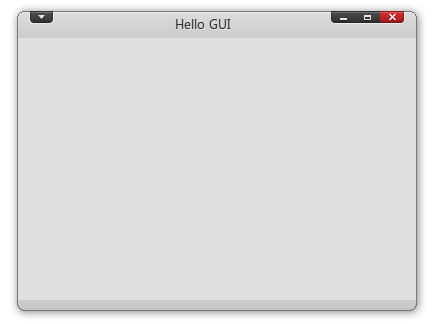
\includegraphics[width=0.6\textwidth]{fig01.png}
%% \end{figure}
% TKS %%%%%%%%%%%%%%%%%%%%%%%%%%%%%%%%%%%%%%%%%%%%%%
\begin{frame}
\centering
{\Huge \textcolor{blue}{THE END}} \\
\vspace{5mm}
{\Large wxd2870@163.com} \\
\end{frame}
%%%%%%%%%%%%%%%%%%%%%%%%%%%%%%%%%%%%%%%%%%%%%%%%%%
\end{document}
